%%
%% This is file `ResearchReport.tex',
%% generated with the docstrip utility.
%%
%% The original source files were:
%%
%% samples.dtx  (with options: `all,proceedings,bibtex,sigconf')
%% 
%% IMPORTANT NOTICE:
%% 
%% For the copyright see the source file.
%% 
%% Any modified versions of this file must be renamed
%% with new filenames distinct from ResearchReport.tex.
%% 
%% For distribution of the original source see the terms
%% for copying and modification in the file samples.dtx.
%% 
%% This generated file may be distributed as long as the
%% original source files, as listed above, are part of the
%% same distribution. (The sources need not necessarily be
%% in the same archive or directory.)
%%
%%
%% Commands for TeXCount
%TC:macro \cite [option:text,text]
%TC:macro \citep [option:text,text]
%TC:macro \citet [option:text,text]
%TC:envir table 0 1
%TC:envir table* 0 1
%TC:envir tabular [ignore] word
%TC:envir displaymath 0 word
%TC:envir math 0 word
%TC:envir comment 0 0
%%
%% The first command in your LaTeX source must be the \documentclass
%% command.
%%
%% For submission and review of your manuscript please change the
%% command to \documentclass[manuscript, screen, review]{acmart}.
%%
%% When submitting camera ready or to TAPS, please change the command
%% to \documentclass[sigconf]{acmart} or whichever template is required
%% for your publication.
%%
%%
\documentclass[sigconf]{acmart}
\usepackage{pdfpages}
\usepackage{graphicx}
\usepackage{afterpage}
\usepackage[abs]{overpic}

\AtBeginDocument{%
  \providecommand\BibTeX{{%
    Bib\TeX}}}

\setcopyright{none}
\renewcommand\footnotetextcopyrightpermission[1]{}
\pagestyle{plain}
\settopmatter{printfolios=true,printccs=false, printacmref=true}

%% Rights management information.  This information is sent to you
%% when you complete the rights form.  These commands have SAMPLE
%% values in them; it is your responsibility as an author to replace
%% the commands and values with those provided to you when you
%% complete the rights form.
% \setcopyright{acmlicensed}

% \copyrightyear{2025}
% \acmYear{2025}
% \acmDOI{XXXXXXX.XXXXXXX}
% %% These commands are for a PROCEEDINGS abstract or paper.
\acmConference[]{Capstone Research Report}{March 2025}{Hamilton, ON, Canada}
% %%
% %%  Uncomment \acmBooktitle if the title of the proceedings is different
% %%  from ``Proceedings of ...''!
% %%
% %%\acmBooktitle{Woodstock '18: ACM Symposium on Neural Gaze Detection,
% %%  June 03--05, 2018, Woodstock, NY}

% \acmISBN{978-1-4503-XXXX-X/2025/06}

%%
%% Submission ID.
%% Use this when submitting an article to a sponsored event. You'll
%% receive a unique submission ID from the organizers
%% of the event, and this ID should be used as the parameter to this command.
%%\acmSubmissionID{123-A56-BU3}

%%
%% For managing citations, it is recommended to use bibliography
%% files in BibTeX format.
%%
%% You can then either use BibTeX with the ACM-Reference-Format style,
%% or BibLaTeX with the acmnumeric or acmauthoryear sytles, that include
%% support for advanced citation of software artefact from the
%% biblatex-software package, also separately available on CTAN.
%%
%% Look at the sample-*-biblatex.tex files for templates showcasing
%% the biblatex styles.
%%

%%
%% The majority of ACM publications use numbered citations and
%% references.  The command \citestyle{authoryear} switches to the
%% "author year" style.
%%
%% If you are preparing content for an event
%% sponsored by ACM SIGGRAPH, you must use the "author year" style of
%% citations and references.
%% Uncommenting
%% the next command will enable that style.
%%\citestyle{acmauthoryear}


%%
%% end of the preamble, start of the body of the document source.
\setcopyright{none}
\makeatletter
\renewcommand\@formatdoi[1]{\ignorespaces}
\makeatother
\begin{document}

%%
%% The "title" command has an optional parameter,
%% allowing the author to define a "short title" to be used in page headers.
\title[Dynamic Memory in Tangled Program Graphs]{Enhancing Reinforcement Learning for MuJoCo Tasks with Dynamic Memory in Tangled Program Graphs}

%%
%% The "author" command and its associated commands are used to define
%% the authors and their affiliations.
%% Of note is the shared affiliation of the first two authors, and the
%% "authornote" and "authornotemark" commands
%% used to denote shared contribution to the research.
\author{Cyruss Allen Amante}
\affiliation{%
  \institution{McMaster University}
  \city{Hamilton}
  \state{Ontario}
  \country{Canada}}
\email{amantec@mcmaster.ca}

\author{Richard Li}
\affiliation{%
  \institution{McMaster University}
  \city{Hamilton}
  \state{Ontario}
  \country{Canada}}
\email{li1502@mcmaster.ca}

\author{Mark Angelo Cruz}
\affiliation{%
  \institution{McMaster University}
  \city{Hamilton}
  \state{Ontario}
  \country{Canada}}
\email{cruzm9@mcmaster.ca}

\author{Calvyn Siong}
\affiliation{%
  \institution{McMaster University}
  \city{Hamilton}
  \state{Ontario}
  \country{Canada}}
\email{siongc1@mcmaster.ca}

\author{Edward Gao}
\affiliation{%
  \institution{McMaster University}
  \city{Hamilton}
  \state{Ontario}
  \country{Canada}}
\email{gaoe2@mcmaster.ca}

%%
%% By default, the full list of authors will be used in the page
%% headers. Often, this list is too long, and will overlap
%% other information printed in the page headers. This command allows
%% the author to define a more concise list
%% of authors' names for this purpose.
% \renewcommand{\shortauthors}{Trovato et al.}

%%
%% The abstract is a short summary of the work to be presented in the
%% article.
\begin{abstract}
  A clear and well-documented \LaTeX\ document is presented as an
  article formatted for publication by ACM in a conference proceedings
  or journal publication. Based on the ``acmart'' document class, this
  article presents and explains many of the common variations, as well
  as many of the formatting elements an author may use in the
  preparation of the documentation of their work.
\end{abstract}

%%
%% The code below is generated by the tool at http://dl.acm.org/ccs.cfm.
%% Please copy and paste the code instead of the example below.
%%
\begin{CCSXML}
<ccs2012>
 <concept>
  <concept_id>00000000.0000000.0000000</concept_id>
  <concept_desc>Do Not Use This Code, Generate the Correct Terms for Your Paper</concept_desc>
  <concept_significance>500</concept_significance>
 </concept>
 <concept>
  <concept_id>00000000.00000000.00000000</concept_id>
  <concept_desc>Do Not Use This Code, Generate the Correct Terms for Your Paper</concept_desc>
  <concept_significance>300</concept_significance>
 </concept>
 <concept>
  <concept_id>00000000.00000000.00000000</concept_id>
  <concept_desc>Do Not Use This Code, Generate the Correct Terms for Your Paper</concept_desc>
  <concept_significance>100</concept_significance>
 </concept>
 <concept>
  <concept_id>00000000.00000000.00000000</concept_id>
  <concept_desc>Do Not Use This Code, Generate the Correct Terms for Your Paper</concept_desc>
  <concept_significance>100</concept_significance>
 </concept>
</ccs2012>
\end{CCSXML}

\ccsdesc[500]{Do Not Use This Code~Generate the Correct Terms for Your Paper}
\ccsdesc[300]{Do Not Use This Code~Generate the Correct Terms for Your Paper}
\ccsdesc{Do Not Use This Code~Generate the Correct Terms for Your Paper}
\ccsdesc[100]{Do Not Use This Code~Generate the Correct Terms for Your Paper}

%%
%% Keywords. The author(s) should pick words that accurately describe
%% the work being presented. Separate the keywords with commas.
\keywords{Do, Not, Us, This, Code, Put, the, Correct, Terms, for,
  Your, Paper}

\received{20 February 2007}
\received[revised]{12 March 2009}
\received[accepted]{5 June 2009}

%%
%% This command processes the author and affiliation and title
%% information and builds the first part of the formatted document.
\maketitle

\section{Introduction}
Reinforcement learning (RL) has emerged as a powerful paradigm for 
training autonomous agents to perform complex tasks. A key challenge 
in RL is creating agents that can generalize to multiple tasks and 
environments, a problem known as multi-task learning (MTL). Real-world 
applications often require agents to adapt to diverse situations, 
making MTL a critical area of research.

Many existing reinforcement learning algorithms struggle with sample 
inefficiency, difficulty in handling continuous control, and poor 
generalization when applied to MuJoCo multi-task learning problems. 
Deep reinforcement learning methods, while powerful, often require vast 
amounts of training data and can be computationally expensive \cite{Mnih07}. These 
methods often fail to capture the temporal dependencies and complex dynamics 
inherent in these environments, leading to sub-optimal performance, especially 
in partially observable scenarios.

\subsection{MuJoCo}
A significant domain for RL research, particularly in robotics, is physics 
simulation. MuJoCo (Multi-Joint dynamics with Contact) is a widely used physics 
engine, known for its accurate and efficient simulation of complex dynamics, 
contact forces, and articulated bodies \cite{Todorov07}. Its ability to simulate realistic 
physics and provide diverse, challenging control tasks makes MuJoCo an invaluable 
tool for developing and evaluating reinforcement learning algorithms for robotics. 
The unique MTL and Single-Task Learning (STL) environments formulated in this work 
includes partially observable versions of the following 6 widely used RL benchmarks 
found on Gymnasium's MuJoCo suite \cite{Towers07}: Ant, Half Cheetah, Hopper, Humanoid Standup, 
Inverted Pendulum, and Inverted Double Pendulum, Figures ~\ref{fig:mujoco_env}(a) to ~\ref{fig:mujoco_env}(e).

\begin{figure}[h]
  \centering
  \begin{tabular}{cc}
    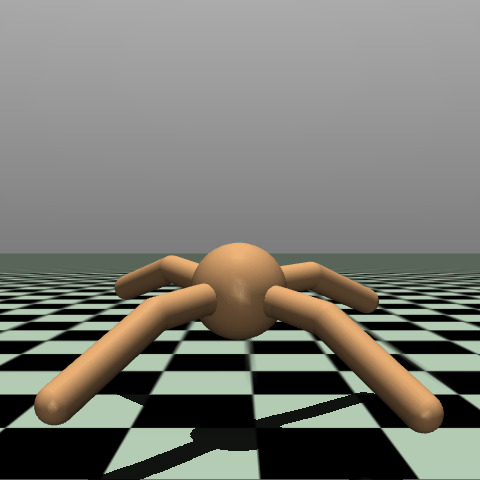
\includegraphics[width=0.3\linewidth]{assets/ant} &
    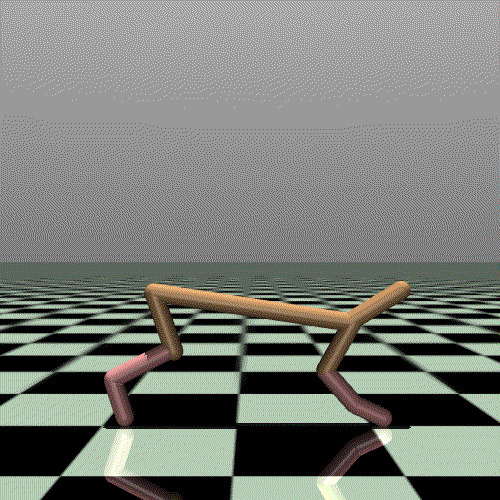
\includegraphics[width=0.3\linewidth]{assets/half_cheetah} \\
    (a) Ant & (b) Half Cheetah \\
    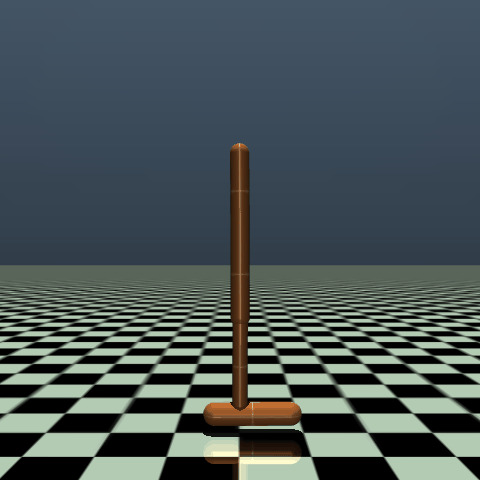
\includegraphics[width=0.3\linewidth]{assets/hopper} &
    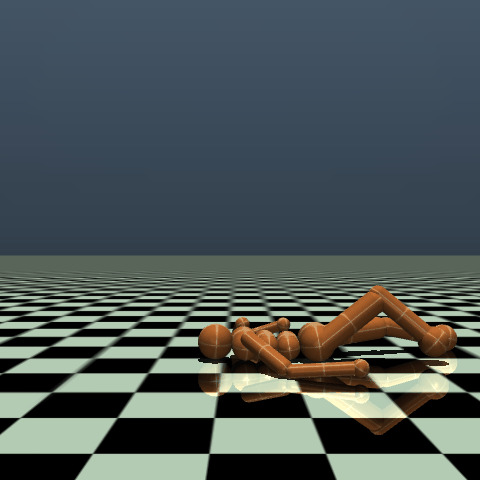
\includegraphics[width=0.3\linewidth]{assets/humanoid_standup} \\
    (c) Hopper & (d) Humanoid Standup \\
    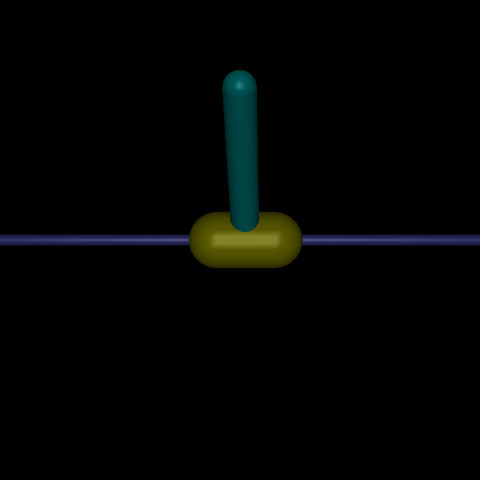
\includegraphics[width=0.3\linewidth]{assets/inverted_pendulum} &
    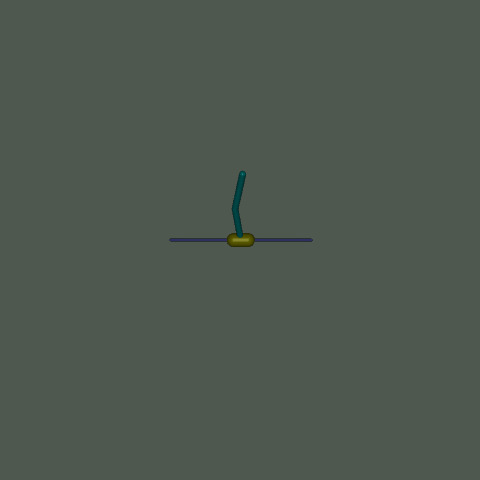
\includegraphics[width=0.3\linewidth]{assets/inverted_double_pendulum} \\
    (e) Inverted Pendulum & (f) Inverted Double Pendulum \\
  \end{tabular}
  \caption{MuJoCo Environments used in this work}
  \label{fig:mujoco_env}
  \Description{MuJoCo Environments used in this work}
\end{figure}

\subsection{Dynamic memory}
Dynamic memory plays a crucial role in evolving program graphs, particularly 
in multi-task learning (MTL), by providing a flexible and adaptive
mechanism for encoding and processing temporal information. Unlike static memory 
architectures, which impose fixed storage structures, dynamic memory allows each 
program within an evolving graph to independently adjust its memory representation 
based on task demands. This adaptability facilitates more efficient learning and 
decision-making, ultimately accelerating evolutionary processes.

Dynamic memory within program graphs consists of three primary types:
\begin{itemize}
  \item \textbf{Scalar Memory}: Stores single numerical values, useful for tracking individual state variables.
  \item \textbf{Vector Memory}: Represents data as structured arrays, allowing operations across multiple related values.
  \item \textbf{Matrix Memory}: Enables higher-dimensional representations, which can encode richer state information 
  and facilitate more complex transformations.
\end{itemize}

Each program selects an appropriate memory type based on its computational needs, 
and mutations can modify both the type and dimensionality of the memory structures over the course of evolution.

\subsection{Tangled Program Graphs}
Tangled Program Graphs (TPG) is an RL framework developed by McMaster University’s Creative Algorithm Lab under the guidance of Dr. Stephen Kelly.
It leverages genetic programming principles to evolve agents capable of solving complex tasks in dynamic environments. Traditional RL methods,
such as deep reinforcement learning (DRL), often rely on neural networks that require significant computational resources and large datasets for training.
~\cite{Winkler2025}  In contrast, TPG uses genetic programming to evolve agents that can learn and adapt to their environment through a process of 
selection, mutation, and crossover. This unique approach allows TPG to achieve competitive performance in RL tasks with better computation
efficiency than DRL methods.~\cite{Winkler2025}

TPG revolves around the concept of emergent modularity, where agents are composed of interconnected programs that map environmental states to actions.
These programs are organized into hierarchical structures, known as program graphs, that allow agents to break complex tasks into simpler subtasks.~\cite{Kelly21} To incorporate TPG with multi-task learning, an agent will have to be trained to perform multiple tasks sequentially.
This is challenging as the agent must balance different objectives and environments while  avoiding catastrophic forgetting
(learning a new task causes agent to forget previously learned tasks, effectively wasting progress).~\cite{Kelly21} TPG’s
hierarchical and modular structure however, is able to tackle this challenge by allowing agents to dynamically adapt to different tasks by 
“recombining specialized behaviors”.~\cite{Kelly21} TPG has been previously used to evolve agents capable of solving six distinct RL benchmarks from OpenAI’s
Classic Control suite, including CartPole, Acrobot, and Pendulum.~\cite{Kelly21} Currently, TPG is being further developed to gauge it’s
capability of integrating multi-task learning with more complex MuJoCo environments.

\section{Motivation}
The primary motivation behind this research and development effort is to enhance the performance and efficiency of TPG in complex environments, specifically within the MuJoCo physics simulation framework. MuJoCo environments, such as Ant, Half Cheetah, and Humanoid Standup, present significant challenges due to their high-dimensional state and action spaces, as well as their dynamic nature. These environments require agents to learn proper control policies that generalize across diverse scenarios, making them ideal benchmarks for evaluating the scalability and adaptability of TPG.

The goal is to both improve performance and increase efficiency. Performance will be measured by the best fitness score achieved by the TPG agent, reflecting its ability to maximize cumulative rewards. Efficiency will be measured by the number of generations required for the agent to converge to an optimal state, which also reflects the time and computational resources needed for training. By integrating dynamic memory and optimizing the evolutionary process, this research aims to reduce the time to learn while maintaining or improving the quality of the learned policies.

\section{Research Questions}

The primary parameter given to the ``\verb|acmart|'' document class is
the {\itshape template style} which corresponds to the kind of publication
or SIG publishing the work. This parameter is enclosed in square
brackets and is a part of the {\verb|documentclass|} command:
\begin{verbatim}
  \documentclass[STYLE]{acmart}
\end{verbatim}

Journals use one of three template styles. All but three ACM journals
use the {\verb|acmsmall|} template style:
\begin{itemize}
\item {\texttt{acmsmall}}: The default journal template style.
\item {\texttt{acmlarge}}: Used by JOCCH and TAP.
\item {\texttt{acmtog}}: Used by TOG.
\end{itemize}

The majority of conference proceedings documentation will use the {\verb|acmconf|} template style.
\begin{itemize}
\item {\texttt{sigconf}}: The default proceedings template style.
\item{\texttt{sigchi}}: Used for SIGCHI conference articles.
\item{\texttt{sigplan}}: Used for SIGPLAN conference articles.
\end{itemize}

\section{Methodology}

This study evaluates task performance parameters such as generation time and 
fitness level through experiments conducted in their respective MuJoCo environments 
(see Figure~\ref{fig:mujoco_env}). The methodology follows a two-phase approach: establishing baselines
and integrating dynamic memory. We compare between baseline and dynamic memory-enhanced
experiments that were conducted using statistical plots and TPG-generated data. All
experiments utilized High Performance Parallel Compute (HPPC) resourcesprovided by the
Digital Research Alliance of Canada (“The Alliance”). Each experiment was run with three
random seeds for a three-hour duration.

\subsection{Baseline Experiments}
We conducted single-task and multi-task experiments using the following MuJoCo environments:
inverted pendulum, inverted double pendulum, and half-cheetah. Single-task experiments used standardized
hyperparameters listed in Table~\ref{tab:hyperparameters}. Each experiment was assigned a specific memory\_size 
parameter value basedon the dimensionality of the observation space, detailed in Table~\ref{tab:observation_space}.

\begin{table*}
  \caption{Hyperparameters for MuJoCo environments, single-task team population, and program population}\label{tab:hyperparameters}
  \centering
  \begin{tabular}{llcllcll}
    \toprule
    \multicolumn{2}{c}{\textbf{MuJoCo parameters}} & & \multicolumn{2}{c}{\textbf{Team population}} & & \multicolumn{2}{c}{\textbf{Program population}} \\
    \cmidrule(r){1-2} \cmidrule(lr){4-5} \cmidrule(l){7-8}
    \textbf{Parameter} & \textbf{Value} & & \textbf{Parameter} & \textbf{Value} & & \textbf{Parameter} & \textbf{Value} \\
    \midrule
    Max timestep & 1000 & & Agent (root team) population size & 1000 & & Initial program size & 10 \\
    Reward control weight & 0.5 & & Initial team size & 1 & & $p_\text{delete}$ & 0.2 \\
    Number of training evaluations & 20 & & Max team size & 10 & & $p_\text{add}$, $p_\text{swap}$, $p_\text{mutate}$ & 0.25 \\
    Number of test evaluations & 1 & & $n\_root\_gen$ & 100 & & $mem_\text{min}$ & 2 \\
    Number of validation evaluations & 0 & & & & & $mem_\text{max}$ & 32 \\
    & & & & & & $p_\text{mem}$ & 0.0 \\
    \bottomrule
  \end{tabular}
  \caption*{\small \textit{Note:} $n\_root\_gen$ denotes the number of new root teams to create each generation. $p_\text{x}$ in which $x \in \{add, delete, swap, mutate\}$ are the probabilities of adding, deleting, swapping, or mutating instructions within a program. $p_\text{mem}$ is the probability of changing the memory size, $mem_\text{size}$, within the $mem_\text{min}$ and $mem_\text{max}$ interval.}
\end{table*}

\begin{table}
  \caption{Observation and action space sizes for the considered problems \cite{FaramaFoundation24}}\label{tab:observation_space}
  \begin{tabular}{lll}
    \toprule
    \textbf{Environment}&\textbf{Obs.}~$\mathcal{O}$&\textbf{Act.}~$\mathcal{A}$\\
    \midrule
    Inverted pendulum & $\mathbb{R}^4$ & [-3, -3]\\
    Inverted double pendulum & $\mathbb{R}^9$ & [-1, 1]\\
    Half cheetah & $\mathbb{R}^{17}$ & [-1, 1]\\
  \bottomrule
\end{tabular}
\end{table}

For multi-task experiments, we utilize the same MuJoCo environments. However, the root team size was increased to 3000,
and $n\_root\_gen$ was increased to 300 to accommodate the added complexity of multi-task learning. Two multi-task
experiments were conducted:

\begin{enumerate}
  \item \textbf{Two-environment multi-task:} Inverted pendulum and inverted double pendulum.
  \item \textbf{Three-environment multi-task:} Inverted pendulum, inverted double pendulum, and half cheetah.
\end{enumerate}

The initial $mem_\text{size}$ parameter was set to 4 for the two-environment multi-task experiment and 17 for the three-environment
multi-task experiment.

\subsection{Dynamic Memory Experiments}
To evaluate the benefits of adaptive memory allocation, we implemented a dynamic memory strategy by increasing the probability
of changing memory size, $p_\text{mem}$, to 10\% (0.1). The effects of this modification were assessed across the same baseline experiments.

\begin{itemize}
  \item For single-task experiments, the minimum and maximum values for $mem_\text{size}$ remained fixed at 2 and 32, respectively.
  \item For multi-task experiments, the minimum and maximum values for $mem_\text{size}$ were dynamically adjusted based on the smallest
  and largest observation space dimensions among the participating environments.
\end{itemize}

\subsection{Data Collection}
For each experiment, performance metrics were systematically recorded and extracted from the \texttt{.std} output files,
then parsed into structured \texttt{.csv} files. These \texttt{.csv} files were categorized into:

\begin{itemize}
  \item \textbf{Timing Metrics:} Measures of computational timing.
  \item \textbf{Selection Metrics:} Data on operations used, fitness level, and instruction count.
  \item \textbf{Replacement Metrics:} Statistics on team and program numbers.
  \item \textbf{Removal Metrics:} Information on program and team deletions.
\end{itemize}

Key performance indicators analyzed include:

\begin{itemize}
  \item \textbf{Best Fitness Score:} The highest fitness score achieved during execution.
  \item \textbf{Generations to Convergence:} The number of generations required to reach a specified performance threshold.
  \item \textbf{Effective Program Instructions:} The number of program instructions contributing to the final output.
\end{itemize}

After data collection, comparative analyses were conducted to evaluate the differences between baseline and dynamic memory configurations
across both single-task and multi-task experiments. Visualization techniques, including comparative plots, were used to identify performance
trends and assess the impact of dynamic memory integration.

\section{Baseline Experiments Results}
This section presents the performance outcomes of the baseline experiments conducted in 
the MuJoCo environments, including single-task and multi-task scenarios. The evaluation 
metrics focus on \textbf{Best Fitness Score} and \textbf{Effective Program Instruction Count}, as illustrated in 
Figures~\ref{fig:best_fitness} and~\ref{fig:effective_program}, respectively.

\subsection{Best Fitness Score Analysis}
The \textbf{Best Fitness Score} metric, depicted in Figure~\ref{fig:best_fitness}, provides insights into the overall 
learning progress of the different experiments. The results highlight several key observations:

\begin{itemize}
  \item \textbf{Single-task environments}: The fitness scores for Half Cheetah and Inverted Pendulum show that while both static and dynamic memory setups improve over time, dynamic memory consistently achieves higher fitness scores faster.
  \item \textbf{Multi-task environments}: Dynamic memory demonstrates a clear advantage, particularly in the Two- and Three-task multi-task setups. It outperforms static memory across generations, highlighting its ability to adapt more effectively to increasing task complexity.
\end{itemize}

\subsection{Program Instruction Count Analysis}
Figure~\ref{fig:effective_program} presents the results of the \textbf{Effective Program Instruction Count}, a key metric reflecting the number of active 
program instructions contributing to task performance.

\begin{itemize}
  \item \textbf{Single-task environments}: Dynamic environments show more fluctuations in active instruction counts, indicating frequent adaptation for optimization. In contrast, static environments stabilize early, limiting flexibility.
  \item \textbf{Multi-task environments}: The Effective Program Instruction Count is significantly higher in dynamic multi-task setups, suggesting better management of complex learning structures. Static environments struggle to scale efficiently.
\end{itemize}

\afterpage{
  \clearpage
  \begin{figure*}[t]
    \centering
    \scalebox{0.87}{
    \begin{tabular}{p{1\linewidth}}
      \begin{overpic}[clip, trim=25 25 125 0, width=0.5\textwidth]{assets/pdf/static/best_fitness/half_cheetah.pdf}
        \put(160,20){\color{black!50}Static Half Cheetah} % Adjust position
        \put(-15,50){\rotatebox{90}{\color{black}\LARGE Best Fitness}} % Adjust position and size
      \end{overpic}
      \begin{overpic}[clip, trim=25 25 125 0, width=0.5\textwidth]{assets/pdf/dynamic/best_fitness/half_cheetah.pdf}
        \put(145,20){\color{black!50}Dynamic Half Cheetah} % Adjust position
      \end{overpic}
    \end{tabular}
    }

    \scalebox{0.87}{
    \begin{tabular}{p{1\linewidth}}
      \begin{overpic}[clip, trim=25 25 125 0, width=0.5\textwidth]{assets/pdf/static/best_fitness/ip.pdf}
        \put(160,20){\color{black!50}\shortstack[r]{Static \\ Inverted Pendulum}} % Adjust position
        \put(-15,50){\rotatebox{90}{\color{black}\LARGE Best Fitness}} % Adjust position and size
      \end{overpic}
      \begin{overpic}[clip, trim=25 25 125 0, width=0.5\textwidth]{assets/pdf/dynamic/best_fitness/ip.pdf}
        \put(160,20){\color{black!50}\shortstack[r]{Dynamic \\ Inverted Pendulum}} % Adjust position
      \end{overpic}
    \end{tabular}
    }

    \scalebox{0.87}{
    \begin{tabular}{p{1\linewidth}}
      \begin{overpic}[clip, trim=25 25 125 0, width=0.5\textwidth]{assets/pdf/static/best_fitness/multitask_general.pdf}
        \put(130,20){\color{black!50}\shortstack[r]{Static \\ Two-Environment Multi-task}} % Adjust position
        \put(-15,50){\rotatebox{90}{\color{black}\LARGE Best Fitness}} % Adjust position and size
      \end{overpic}
      \begin{overpic}[clip, trim=25 25 125 0, width=0.5\textwidth]{assets/pdf/dynamic/best_fitness/multitask_general.pdf}
        \put(125,20){\color{black!50}\shortstack[r]{Dynamic \\ Two-Environment Multi-task}} % Adjust position
      \end{overpic}
    \end{tabular}
    }

    \scalebox{0.87}{
    \begin{tabular}{p{1\linewidth}}
      \begin{overpic}[clip, trim=25 25 125 0, width=0.5\textwidth]{assets/pdf/static/best_fitness/multitask_hc.pdf}
        \put(125,20){\color{black!50}\shortstack[r]{Static \\ Three-Environment Multi-task}} % Adjust position
        \put(-15,50){\rotatebox{90}{\color{black}\LARGE Best Fitness}} % Adjust position and size
      \end{overpic}
      \begin{overpic}[clip, trim=25 25 125 0, width=0.5\textwidth]{assets/pdf/dynamic/best_fitness/multitask_hc.pdf}
        \put(120,20){\color{black!50}\shortstack[r]{Dynamic \\ Three-Environment Multi-task}} % Adjust position
      \end{overpic}
    \end{tabular}
    }
    
    \caption{Best Fitness Score results from Single and Multi-task Baseline Experiments}
    \label{fig:best_fitness}
  \end{figure*}
  
  \clearpage
}
\afterpage{
  \clearpage
  \begin{figure*}[t]
    \centering
    \scalebox{0.87}{
    \begin{tabular}{p{1\linewidth}}
      \begin{overpic}[clip, trim=25 25 125 0, width=0.5\textwidth]{assets/pdf/static/effective_program_instruction_count/half_cheetah.pdf}
        \put(160,20){\color{black!50}Static Half Cheetah} % Adjust position
        \put(-15,20){\rotatebox{90}{\color{black}\LARGE Effective Instruction Count}} % Adjust position and size
      \end{overpic}
      \begin{overpic}[clip, trim=25 25 125 0, width=0.5\textwidth]{assets/pdf/dynamic/effective_program_instruction_count/half_cheetah.pdf}
        \put(145,20){\color{black!50}Dynamic Half Cheetah} % Adjust position
      \end{overpic}
    \end{tabular}
    }

    \scalebox{0.87}{
    \begin{tabular}{p{1\linewidth}}
      \begin{overpic}[clip, trim=25 25 125 0, width=0.5\textwidth]{assets/pdf/static/effective_program_instruction_count/ip.pdf}
        \put(160,20){\color{black!50}\shortstack[r]{Static \\ Inverted Pendulum}} % Adjust position
        \put(-15,20){\rotatebox{90}{\color{black}\LARGE Effective Instruction Count}} % Adjust position and size
      \end{overpic}
      \begin{overpic}[clip, trim=25 25 125 0, width=0.5\textwidth]{assets/pdf/dynamic/effective_program_instruction_count/ip.pdf}
        \put(160,20){\color{black!50}\shortstack[r]{Dynamic \\ Inverted Pendulum}} % Adjust position
      \end{overpic}
    \end{tabular}
    }

    \scalebox{0.87}{
    \begin{tabular}{p{1\linewidth}}
      \begin{overpic}[clip, trim=25 25 125 0, width=0.5\textwidth]{assets/pdf/static/effective_program_instruction_count/multitask_general.pdf}
        \put(130,20){\color{black!50}\shortstack[r]{Static \\ Two-Environment Multi-task}} % Adjust position
        \put(-15,20){\rotatebox{90}{\color{black}\LARGE Effective Instruction Count}} % Adjust position and size
      \end{overpic}
      \begin{overpic}[clip, trim=25 25 125 0, width=0.5\textwidth]{assets/pdf/dynamic/effective_program_instruction_count/multitask_general.pdf}
        \put(125,20){\color{black!50}\shortstack[r]{Dynamic \\ Two-Environment Multi-task}} % Adjust position
      \end{overpic}
    \end{tabular}
    }

    \scalebox{0.87}{
    \begin{tabular}{p{1\linewidth}}
      \begin{overpic}[clip, trim=25 25 125 0, width=0.5\textwidth]{assets/pdf/static/effective_program_instruction_count/multitask_hc.pdf}
        \put(125,20){\color{black!50}\shortstack[r]{Static \\ Three-Environment Multi-task}} % Adjust position
        \put(-15,20){\rotatebox{90}{\color{black}\LARGE Effective Instruction Count}} % Adjust position and size
      \end{overpic}
      \begin{overpic}[clip, trim=25 25 125 0, width=0.5\textwidth]{assets/pdf/dynamic/effective_program_instruction_count/multitask_hc.pdf}
        \put(120,20){\color{black!50}\shortstack[r]{Dynamic \\ Three-Environment Multitask}} % Adjust position
      \end{overpic}
    \end{tabular}
    }
    
    \caption{Effective Program Instruction Count results from Single and Multi-task Baseline Experiments}\label{fig:effective_program}
  \end{figure*}

  \clearpage
}

\section{Typefaces}

The ``\verb|acmart|'' document class requires the use of the
``Libertine'' typeface family. Your \TeX\ installation should include
this set of packages. Please do not substitute other typefaces. The
``\verb|lmodern|'' and ``\verb|ltimes|'' packages should not be used,
as they will override the built-in typeface families.

\section{Title Information}

The title of your work should use capital letters appropriately -
\url{https://capitalizemytitle.com/} has useful rules for
capitalization. Use the {\verb|title|} command to define the title of
your work. If your work has a subtitle, define it with the
{\verb|subtitle|} command.  Do not insert line breaks in your title.

If your title is lengthy, you must define a short version to be used
in the page headers, to prevent overlapping text. The \verb|title|
command has a ``short title'' parameter:
\begin{verbatim}
  \title[short title]{full title}
\end{verbatim}

\section{Authors and Affiliations}

Each author must be defined separately for accurate metadata
identification.  As an exception, multiple authors may share one
affiliation. Authors' names should not be abbreviated; use full first
names wherever possible. Include authors' e-mail addresses whenever
possible.

Grouping authors' names or e-mail addresses, or providing an ``e-mail
alias,'' as shown below, is not acceptable:
\begin{verbatim}
  \author{Brooke Aster, David Mehldau}
  \email{dave,judy,steve@university.edu}
  \email{firstname.lastname@phillips.org}
\end{verbatim}

The \verb|authornote| and \verb|authornotemark| commands allow a note
to apply to multiple authors --- for example, if the first two authors
of an article contributed equally to the work.

If your author list is lengthy, you must define a shortened version of
the list of authors to be used in the page headers, to prevent
overlapping text. The following command should be placed just after
the last \verb|\author{}| definition:
\begin{verbatim}
  \renewcommand{\shortauthors}{McCartney, et al.}
\end{verbatim}
Omitting this command will force the use of a concatenated list of all
of the authors' names, which may result in overlapping text in the
page headers.

The article template's documentation, available at
\url{https://www.acm.org/publications/proceedings-template}, has a
complete explanation of these commands and tips for their effective
use.

Note that authors' addresses are mandatory for journal articles.

\section{Rights Information}

Authors of any work published by ACM will need to complete a rights
form. Depending on the kind of work, and the rights management choice
made by the author, this may be copyright transfer, permission,
license, or an OA (open access) agreement.

Regardless of the rights management choice, the author will receive a
copy of the completed rights form once it has been submitted. This
form contains \LaTeX\ commands that must be copied into the source
document. When the document source is compiled, these commands and
their parameters add formatted text to several areas of the final
document:
\begin{itemize}
\item the ``ACM Reference Format'' text on the first page.
\item the ``rights management'' text on the first page.
\item the conference information in the page header(s).
\end{itemize}

Rights information is unique to the work; if you are preparing several
works for an event, make sure to use the correct set of commands with
each of the works.

The ACM Reference Format text is required for all articles over one
page in length, and is optional for one-page articles (abstracts).

\section{CCS Concepts and User-Defined Keywords}

Two elements of the ``acmart'' document class provide powerful
taxonomic tools for you to help readers find your work in an online
search.

The ACM Computing Classification System ---
\url{https://www.acm.org/publications/class-2012} --- is a set of
classifiers and concepts that describe the computing
discipline. Authors can select entries from this classification
system, via \url{https://dl.acm.org/ccs/ccs.cfm}, and generate the
commands to be included in the \LaTeX\ source.

User-defined keywords are a comma-separated list of words and phrases
of the authors' choosing, providing a more flexible way of describing
the research being presented.

CCS concepts and user-defined keywords are required for for all
articles over two pages in length, and are optional for one- and
two-page articles (or abstracts).

\section{Sectioning Commands}

Your work should use standard \LaTeX\ sectioning commands:
\verb|\section|, \verb|\subsection|, \verb|\subsubsection|,
\verb|\paragraph|, and \verb|\subparagraph|. The sectioning levels up to
\verb|\subsusection| should be numbered; do not remove the numbering
from the commands.

Simulating a sectioning command by setting the first word or words of
a paragraph in boldface or italicized text is {\bfseries not allowed.}

Below are examples of sectioning commands.

\subsection{Subsection}
\label{sec:subsection}

This is a subsection.

\subsubsection{Subsubsection}
\label{sec:subsubsection}

This is a subsubsection.

\paragraph{Paragraph}

This is a paragraph.

\subparagraph{Subparagraph}

This is a subparagraph.

\section{Tables}

The ``\verb|acmart|'' document class includes the ``\verb|booktabs|''
package --- \url{https://ctan.org/pkg/booktabs} --- for preparing
high-quality tables.

Table captions are placed {\itshape above} the table.

Because tables cannot be split across pages, the best placement for
them is typically the top of the page nearest their initial cite.  To
ensure this proper ``floating'' placement of tables, use the
environment \textbf{table} to enclose the table's contents and the
table caption.  The contents of the table itself must go in the
\textbf{tabular} environment, to be aligned properly in rows and
columns, with the desired horizontal and vertical rules.  Again,
detailed instructions on \textbf{tabular} material are found in the
\textit{\LaTeX\ User's Guide}.

Immediately following this sentence is the point at which
Table~\ref{tab:freq} is included in the input file; compare the
placement of the table here with the table in the printed output of
this document.

\begin{table}
  \caption{Frequency of Special Characters}
  \label{tab:freq}
  \begin{tabular}{ccl}
    \toprule
    Non-English or Math&Frequency&Comments\\
    \midrule
    \O & 1 in 1,000& For Swedish names\\
    $\pi$ & 1 in 5& Common in math\\
    \$ & 4 in 5 & Used in business\\
    $\Psi^2_1$ & 1 in 40,000& Unexplained usage\\
  \bottomrule
\end{tabular}
\end{table}

To set a wider table, which takes up the whole width of the page's
live area, use the environment \textbf{table*} to enclose the table's
contents and the table caption.  As with a single-column table, this
wide table will ``float'' to a location deemed more
desirable. Immediately following this sentence is the point at which
Table~\ref{tab:commands} is included in the input file; again, it is
instructive to compare the placement of the table here with the table
in the printed output of this document.

\begin{table*}
  \caption{Some Typical Commands}
  \label{tab:commands}
  \begin{tabular}{ccl}
    \toprule
    Command &A Number & Comments\\
    \midrule
    \texttt{{\char'134}author} & 100& Author \\
    \texttt{{\char'134}table}& 300 & For tables\\
    \texttt{{\char'134}table*}& 400& For wider tables\\
    \bottomrule
  \end{tabular}
\end{table*}

Always use midrule to separate table header rows from data rows, and
use it only for this purpose. This enables assistive technologies to
recognise table headers and support their users in navigating tables
more easily.

\section{Math Equations}
You may want to display math equations in three distinct styles:
inline, numbered or non-numbered display.  Each of the three are
discussed in the next sections.

\subsection{Inline (In-text) Equations}
A formula that appears in the running text is called an inline or
in-text formula.  It is produced by the \textbf{math} environment,
which can be invoked with the usual
\texttt{{\char'134}begin\,\ldots{\char'134}end} construction or with
the short form \texttt{\$\,\ldots\$}. You can use any of the symbols
and structures, from $\alpha$ to $\omega$, available in
examples of in-text equations in context. Notice how this equation:
\begin{math}
  \lim_{n\rightarrow \infty}x=0
\end{math},
set here in in-line math style, looks slightly different when
set in display style.  (See next section).

\subsection{Display Equations}
A numbered display equation---one set off by vertical space from the
text and centered horizontally---is produced by the \textbf{equation}
environment. An unnumbered display equation is produced by the
\textbf{displaymath} environment.

Again, in either environment, you can use any of the symbols and
structures available in \LaTeX\@; this section will just give a couple
of examples of display equations in context.  First, consider the
equation, shown as an inline equation above:
\begin{equation}
  \lim_{n\rightarrow \infty}x=0
\end{equation}
Notice how it is formatted somewhat differently in
the \textbf{displaymath}
environment.  Now, we'll enter an unnumbered equation:
\begin{displaymath}
  \sum_{i=0}^{\infty} x + 1
\end{displaymath}
and follow it with another numbered equation:
\begin{equation}
  \sum_{i=0}^{\infty}x_i=\int_{0}^{\pi+2} f
\end{equation}
just to demonstrate \LaTeX's able handling of numbering.

\section{Figures}

The ``\verb|figure|'' environment should be used for figures. One or
more images can be placed within a figure. If your figure contains
third-party material, you must clearly identify it as such, as shown
in the example below.
\begin{figure}[h]
  \centering
  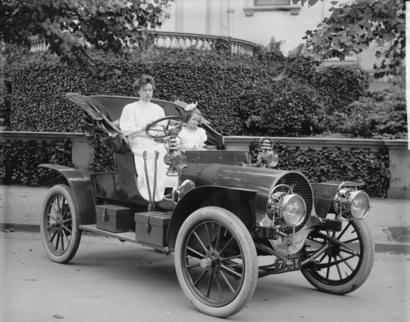
\includegraphics[width=\linewidth]{assets/sample-franklin}
  \caption{1907 Franklin Model D roadster. Photograph by Harris \&
    Ewing, Inc. [Public domain], via Wikimedia
    Commons. (\url{https://goo.gl/VLCRBB}).}
  \Description{A woman and a girl in white dresses sit in an open car.}
\end{figure}

Your figures should contain a caption which describes the figure to
the reader.

Figure captions are placed {\itshape below} the figure.

Every figure should also have a figure description unless it is purely
decorative. These descriptions convey what’s in the image to someone
who cannot see it. They are also used by search engine crawlers for
indexing images, and when images cannot be loaded.

A figure description must be unformatted plain text less than 2000
characters long (including spaces).  {\bfseries Figure descriptions
  should not repeat the figure caption – their purpose is to capture
  important information that is not already provided in the caption or
  the main text of the paper.} For figures that convey important and
complex new information, a short text description may not be
adequate. More complex alternative descriptions can be placed in an
appendix and referenced in a short figure description. For example,
provide a data table capturing the information in a bar chart, or a
structured list representing a graph.  For additional information
regarding how best to write figure descriptions and why doing this is
so important, please see
\url{https://www.acm.org/publications/taps/describing-figures/}.

\subsection{The ``Teaser Figure''}

A ``teaser figure'' is an image, or set of images in one figure, that
are placed after all author and affiliation information, and before
the body of the article, spanning the page. If you wish to have such a
figure in your article, place the command immediately before the
\verb|\maketitle| command:
\begin{verbatim}
  \begin{teaserfigure}
    \includegraphics[width=\textwidth]{sampleteaser}
    \caption{figure caption}
    \Description{figure description}
  \end{teaserfigure}
\end{verbatim}

\section{Citations and Bibliographies}

The use of \BibTeX\ for the preparation and formatting of one's
references is strongly recommended. Authors' names should be complete
--- use full first names (``Donald E. Knuth'') not initials
(``D. E. Knuth'') --- and the salient identifying features of a
reference should be included: title, year, volume, number, pages,
article DOI, etc.

The bibliography is included in your source document with these two
commands, placed just before the \verb|\end{document}| command:
\begin{verbatim}
  \bibliographystyle{ACM-Reference-Format}
  \bibliography{bibfile}
\end{verbatim}
where ``\verb|bibfile|'' is the name, without the ``\verb|.bib|''
suffix, of the \BibTeX\ file.

Citations and references are numbered by default. A small number of
ACM publications have citations and references formatted in the
``author year'' style; for these exceptions, please include this
command in the {\bfseries preamble} (before the command
``\verb|\begin{document}|'') of your \LaTeX\ source:
\begin{verbatim}
  \citestyle{acmauthoryear}
\end{verbatim}


  % Some examples.  A paginated journal article \cite{Abril07}, an
  % enumerated journal article \cite{Cohen07}, a reference to an entire
  % issue \cite{JCohen96}, a monograph (whole book) \cite{Kosiur01}, a
  % monograph/whole book in a series (see 2a in spec. document)
  % \cite{Harel79}, a divisible-book such as an anthology or compilation
  % \cite{Editor00} followed by the same example, however we only output
  % the series if the volume number is given \cite{Editor00a} (so
  % Editor00a's series should NOT be present since it has no vol. no.),
  % a chapter in a divisible book \cite{Spector90}, a chapter in a
  % divisible book in a series \cite{Douglass98}, a multi-volume work as
  % book \cite{Knuth97}, a couple of articles in a proceedings (of a
  % conference, symposium, workshop for example) (paginated proceedings
  % article) \cite{Andler79, Hagerup1993}, a proceedings article with
  % all possible elements \cite{Smith10}, an example of an enumerated
  % proceedings article \cite{VanGundy07}, an informally published work
  % \cite{Harel78}, a couple of preprints \cite{Bornmann2019,
  %   AnzarootPBM14}, a doctoral dissertation \cite{Clarkson85}, a
  % master's thesis: \cite{anisi03}, an online document / world wide web
  % resource \cite{Thornburg01, Ablamowicz07, Poker06}, a video game
  % (Case 1) \cite{Obama08} and (Case 2) \cite{Novak03} and \cite{Lee05}
  % and (Case 3) a patent \cite{JoeScientist001}, work accepted for
  % publication \cite{rous08}, 'YYYYb'-test for prolific author
  % \cite{SaeediMEJ10} and \cite{SaeediJETC10}. Other cites might
  % contain 'duplicate' DOI and URLs (some SIAM articles)
  % \cite{Kirschmer:2010:AEI:1958016.1958018}. Boris / Barbara Beeton:
  % multi-volume works as books \cite{MR781536} and \cite{MR781537}. A
  % couple of citations with DOIs:
  % \cite{2004:ITE:1009386.1010128,Kirschmer:2010:AEI:1958016.1958018}. Online
  % citations: \cite{TUGInstmem, Thornburg01, CTANacmart}.
  % Artifacts: \cite{R} and \cite{UMassCitations}.

\section{Acknowledgments}

Identification of funding sources and other support, and thanks to
individuals and groups that assisted in the research and the
preparation of the work should be included in an acknowledgment
section, which is placed just before the reference section in your
document.

This section has a special environment:
\begin{verbatim}
  \begin{acks}
  ...
  \end{acks}
\end{verbatim}
so that the information contained therein can be more easily collected
during the article metadata extraction phase, and to ensure
consistency in the spelling of the section heading.

Authors should not prepare this section as a numbered or unnumbered {\verb|\section|}; please use the ``{\verb|acks|}'' environment.

\section{Appendices}

If your work needs an appendix, add it before the
``\verb|\end{document}|'' command at the conclusion of your source
document.

Start the appendix with the ``\verb|appendix|'' command:
\begin{verbatim}
  \appendix
\end{verbatim}
and note that in the appendix, sections are lettered, not
numbered. This document has two appendices, demonstrating the section
and subsection identification method.

\section{Multi-language papers}

Papers may be written in languages other than English or include
titles, subtitles, keywords and abstracts in different languages (as a
rule, a paper in a language other than English should include an
English title and an English abstract).  Use \verb|language=...| for
every language used in the paper.  The last language indicated is the
main language of the paper.  For example, a French paper with
additional titles and abstracts in English and German may start with
the following command
\begin{verbatim}
\documentclass[sigconf, language=english, language=german,
               language=french]{acmart}
\end{verbatim}

The title, subtitle, keywords and abstract will be typeset in the main
language of the paper.  The commands \verb|\translatedXXX|, \verb|XXX|
begin title, subtitle and keywords, can be used to set these elements
in the other languages.  The environment \verb|translatedabstract| is
used to set the translation of the abstract.  These commands and
environment have a mandatory first argument: the language of the
second argument.  See \verb|sample-sigconf-i13n.tex| file for examples
of their usage.

\section{SIGCHI Extended Abstracts}

The ``\verb|sigchi-a|'' template style (available only in \LaTeX\ and
not in Word) produces a landscape-orientation formatted article, with
a wide left margin. Three environments are available for use with the
``\verb|sigchi-a|'' template style, and produce formatted output in
the margin:
\begin{description}
\item[\texttt{sidebar}:]  Place formatted text in the margin.
\item[\texttt{marginfigure}:] Place a figure in the margin.
\item[\texttt{margintable}:] Place a table in the margin.
\end{description}

%%
%% The acknowledgments section is defined using the "acks" environment
%% (and NOT an unnumbered section). This ensures the proper
%% identification of the section in the article metadata, and the
%% consistent spelling of the heading.
\begin{acks}
To Dr. Stephen Kelly, for guiding us throughout the research process and providing valuable insights and feedback.
\end{acks}

%%
%% The next two lines define the bibliography style to be used, and
%% the bibliography file.
\bibliographystyle{assets/ACM-Reference-Format}
\bibliography{assets/research-base}


%%
%% If your work has an appendix, this is the place to put it.
\appendix

\section{Research Methods}

\subsection{Part One}

Lorem ipsum dolor sit amet, onsectetur adipiscing elit. Morbi
malesuada, quam in pulvinar varius, metus nunc fermentum urna, id
sollicitudin purus odio sit amet enim. Aliquam ullamcorper eu ipsum
vel mollis. Curabitur quis dictum nisl. Phasellus vel semper risus, et
lacinia dolor. Integer ultricies commodo sem nec semper.

\subsection{Part Two}

Etiam commodo feugiat nisl pulvinar pellentesque. Etiam auctor sodales
ligula, non varius nibh pulvinar semper. Suspendisse nec lectus non
ipsum convallis congue hendrerit vitae sapien. Donec at laoreet
eros. Vivamus non purus placerat, scelerisque diam eu, cursus
ante. Etiam aliquam tortor auctor efficitur mattis.

\section{Online Resources}

Nam id fermentum dui. Suspendisse sagittis tortor a nulla mollis, in
pulvinar ex pretium. Sed interdum orci quis metus euismod, et sagittis
enim maximus. Vestibulum gravida massa ut felis suscipit
congue. Quisque mattis elit a risus ultrices commodo venenatis eget
dui. Etiam sagittis eleifend elementum.

Nam interdum magna at lectus dignissim, ac dignissim lorem
rhoncus. Maecenas eu arcu ac neque placerat aliquam. Nunc pulvinar
massa et mattis lacinia.

\end{document}
\endinput
%%
%% End of file `ResearchReport.tex'.
